\section{Part B - Analysis and Controller Design}%
\label{b}


Henceforth, a set of values are assumed to carry out simulations : $m = 0.425kg$, $g=9.81m/s^2$, $d = 0.42m$, $\delta = 0.65m$, $r = 0.125m$, $R = 53\omega$, $L_{0} = 120mH$, $L_{1} = 25mH$, $\alpha = 1.2m^-1$, $c = 6815_{A^2 \cdot s^2}^{g\cdot m^3}$, $ k = 1880N/m$, $b = 10.4Ns/m$, $\phi = 42^{\circ} \\ 

\textbf{B1} \\
\textbf{B2} \\ 
\textbf{B3} \\ 

\begin{figure}[H]
	\centering
	\captionsetup{justification=centering}
	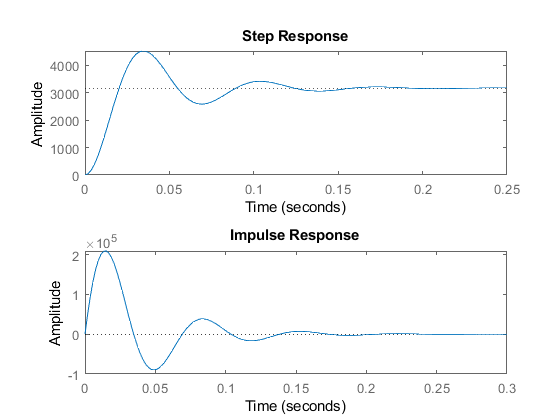
\includegraphics[width=1\linewidth]{imgs/Impulse step response.png}
	\caption{Position over time}%
	\label{fig:14}
\end{figure}

\textbf{B4} \\ 

\begin{figure}[H]
	\centering
	\captionsetup{justification=centering}
	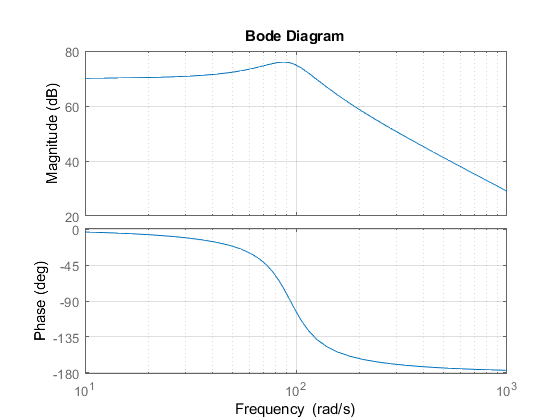
\includegraphics[width=1\linewidth]{imgs/Bode plot.png}
	\caption{Position over time}%
	\label{fig:14}
\end{figure}

\textbf{B5} \\ 